\newpage
\section*{Domain Discovery}

Using the directionality indices computed on at 10kb resolution map, we computed domains by selecting the regions with the top
$10\%$ directionality bias.  Domains were further refined by intersecting between replicates and discarding non-overlapping
domains, leaving a small, conserved subset.  Overlaps between window sizes and replicates are shown in the figures below.

\subsection*{Domain Conservation}

\begin{figure}[thb]
  \centering
  \caption{Conserved Domains between IMR90 Replicates}
  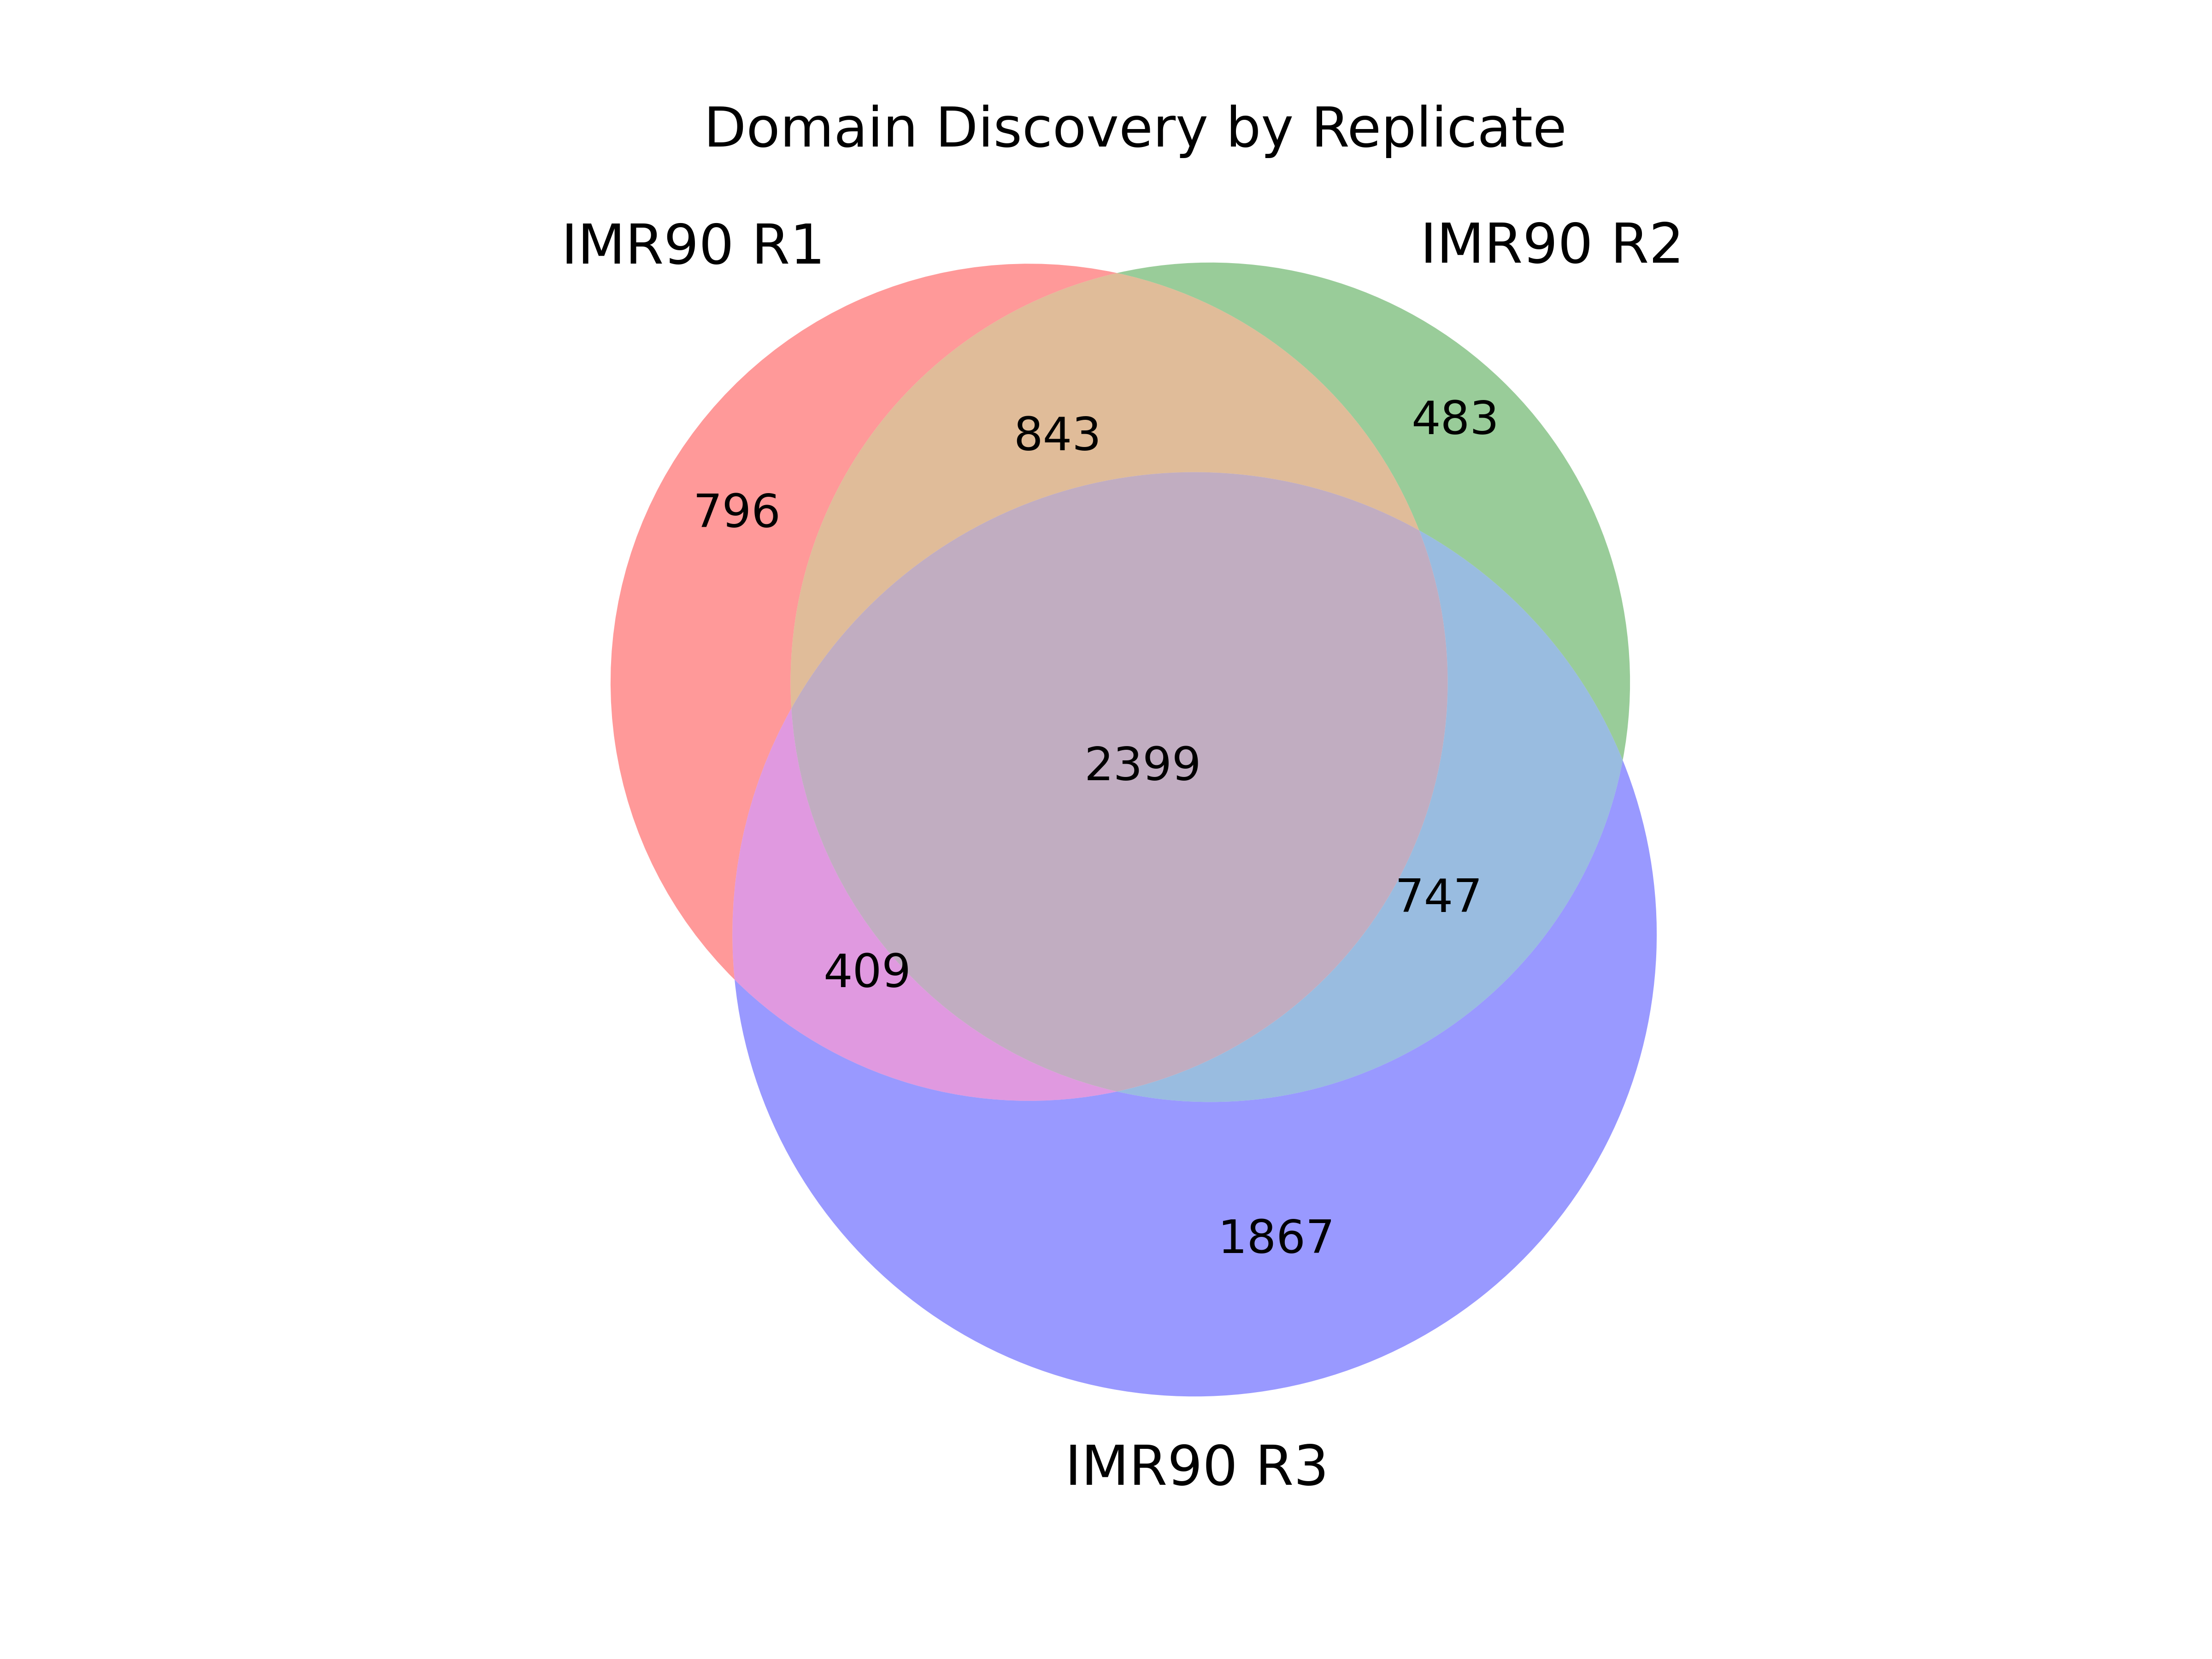
\includegraphics[width=\textwidth]{figures/supplementary/domains/venn3.png}\label{fig:SuppVenn3}
\end{figure}

\begin{figure}[thp]
  \caption{Domain Overlaps by Window Size}
  \begin{minipage}{0.45\textwidth}%
    \centering
    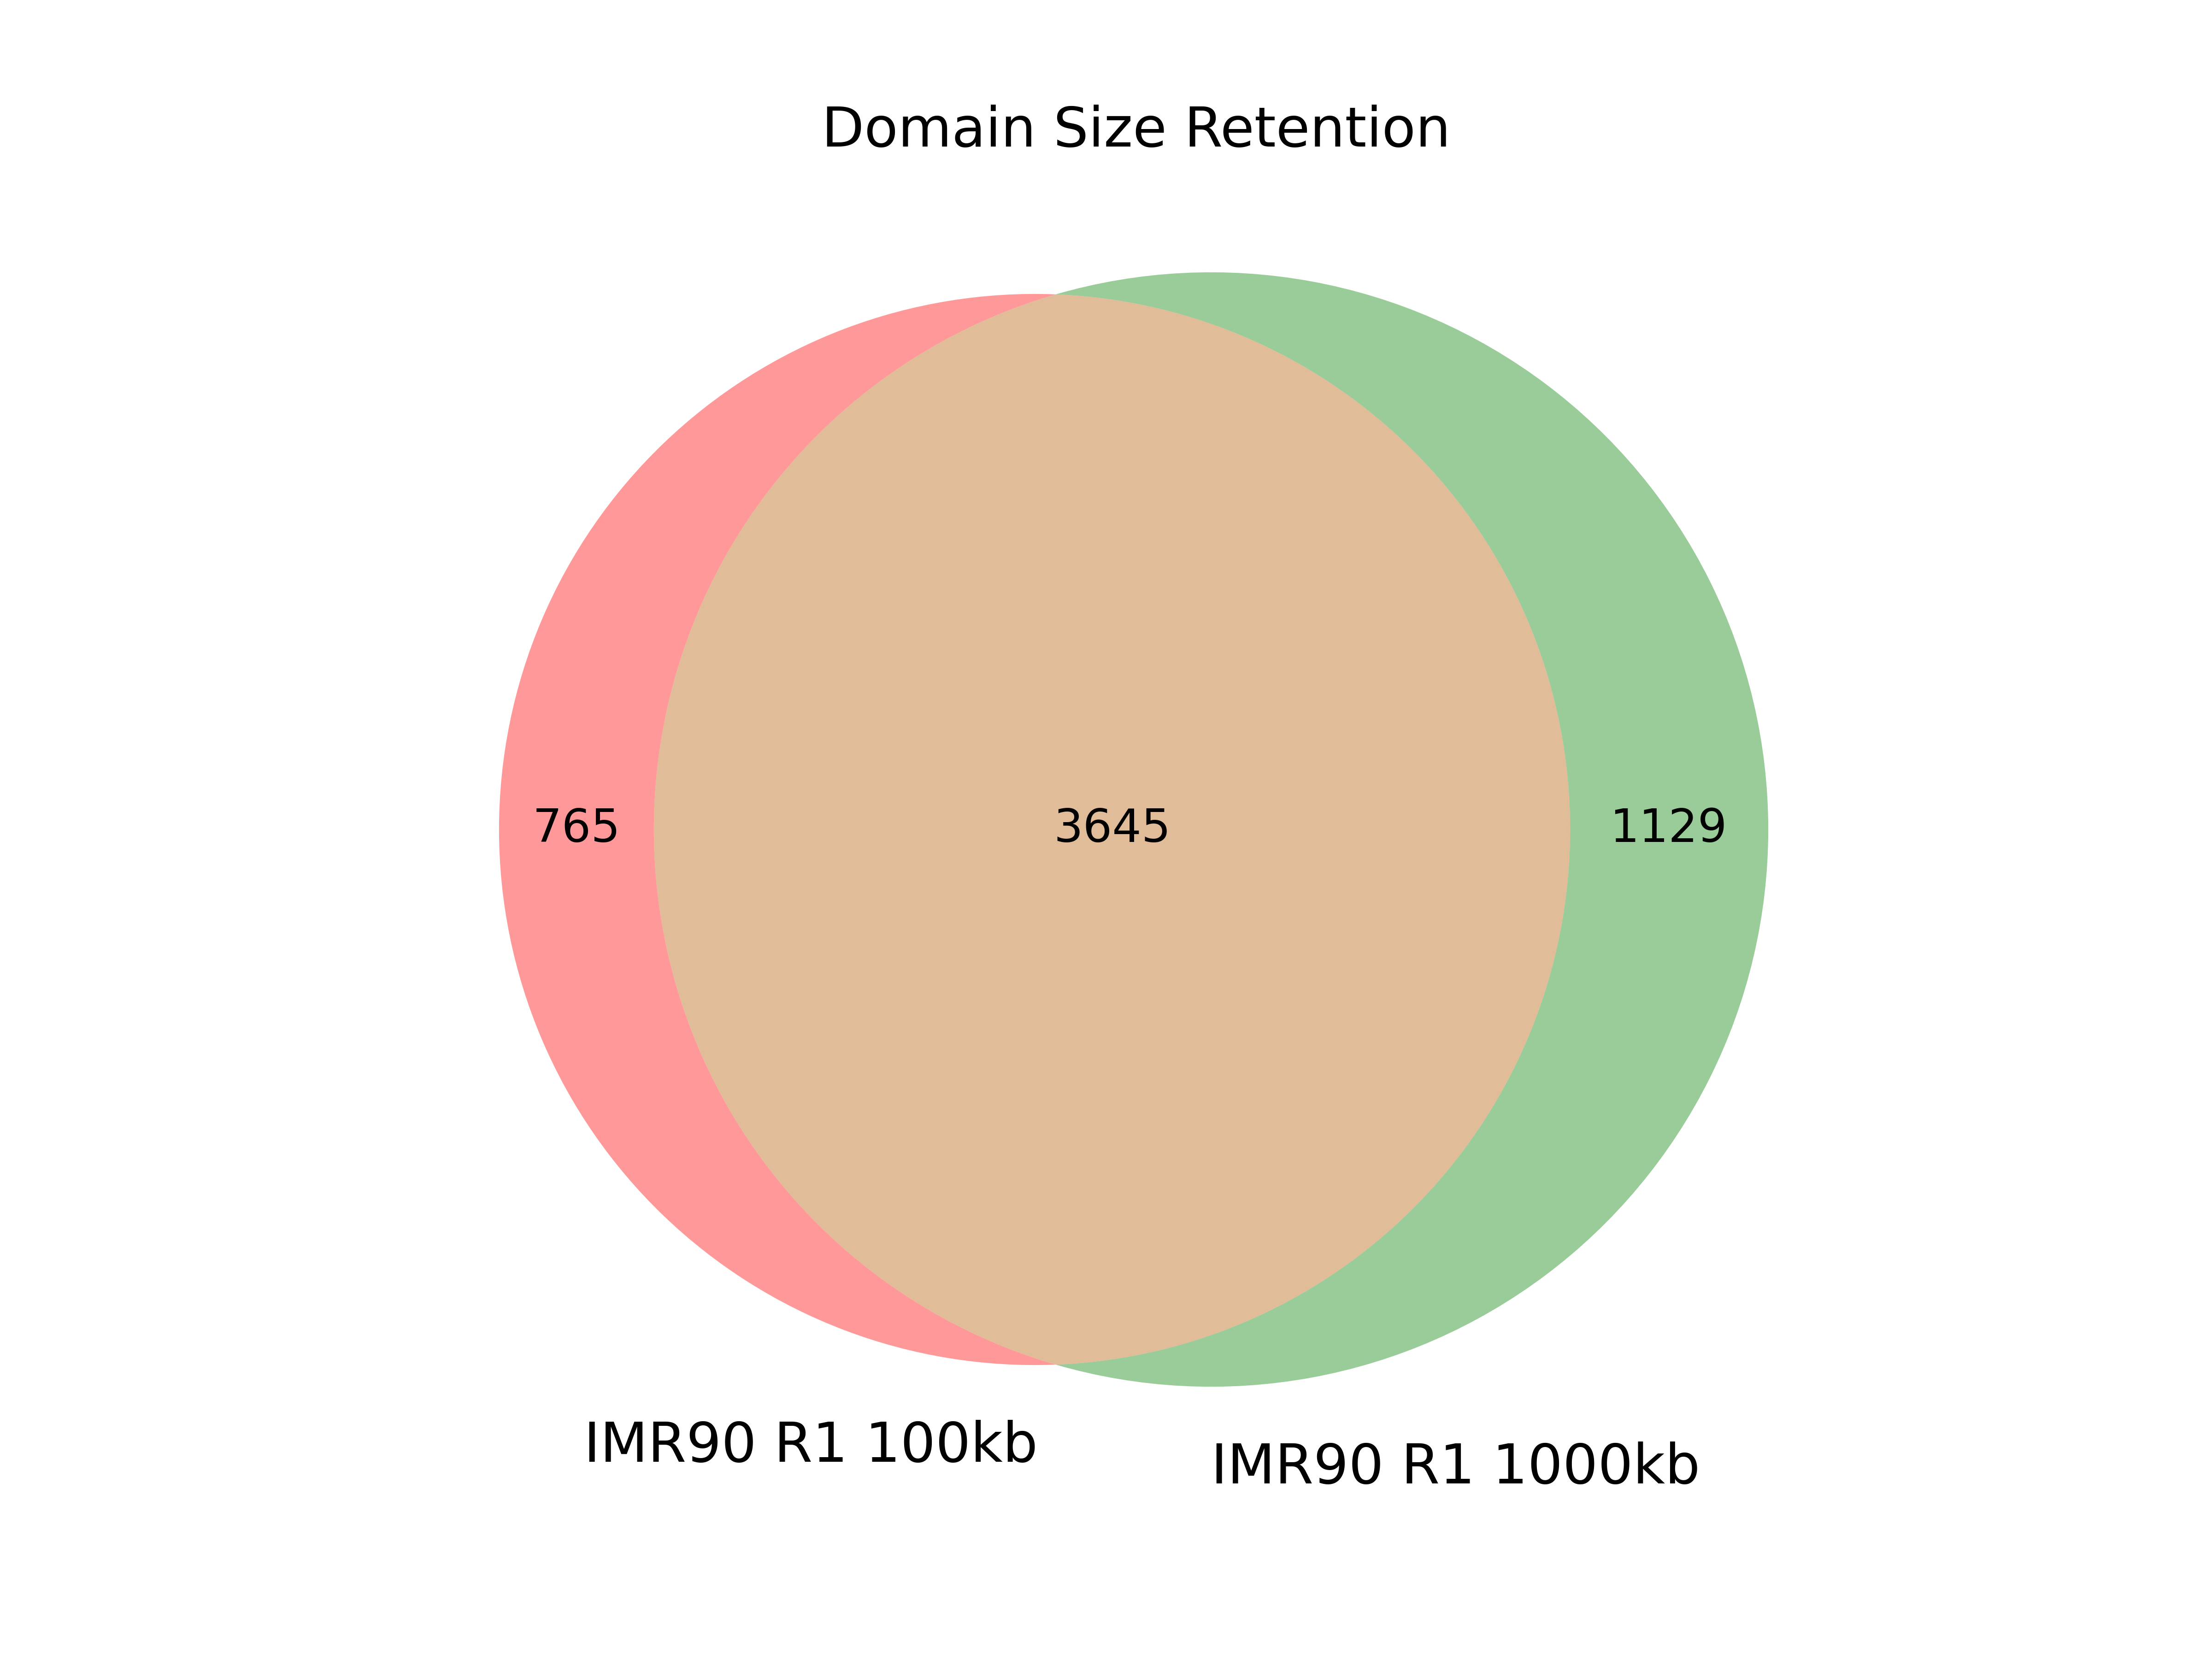
\includegraphics[width=\textwidth]{./figures/supplementary/domains/venn2_ir1_100kb_vs_ir1_1000kb.png}
  \end{minipage}

  \begin{minipage}{0.45\textwidth}
    \centering
    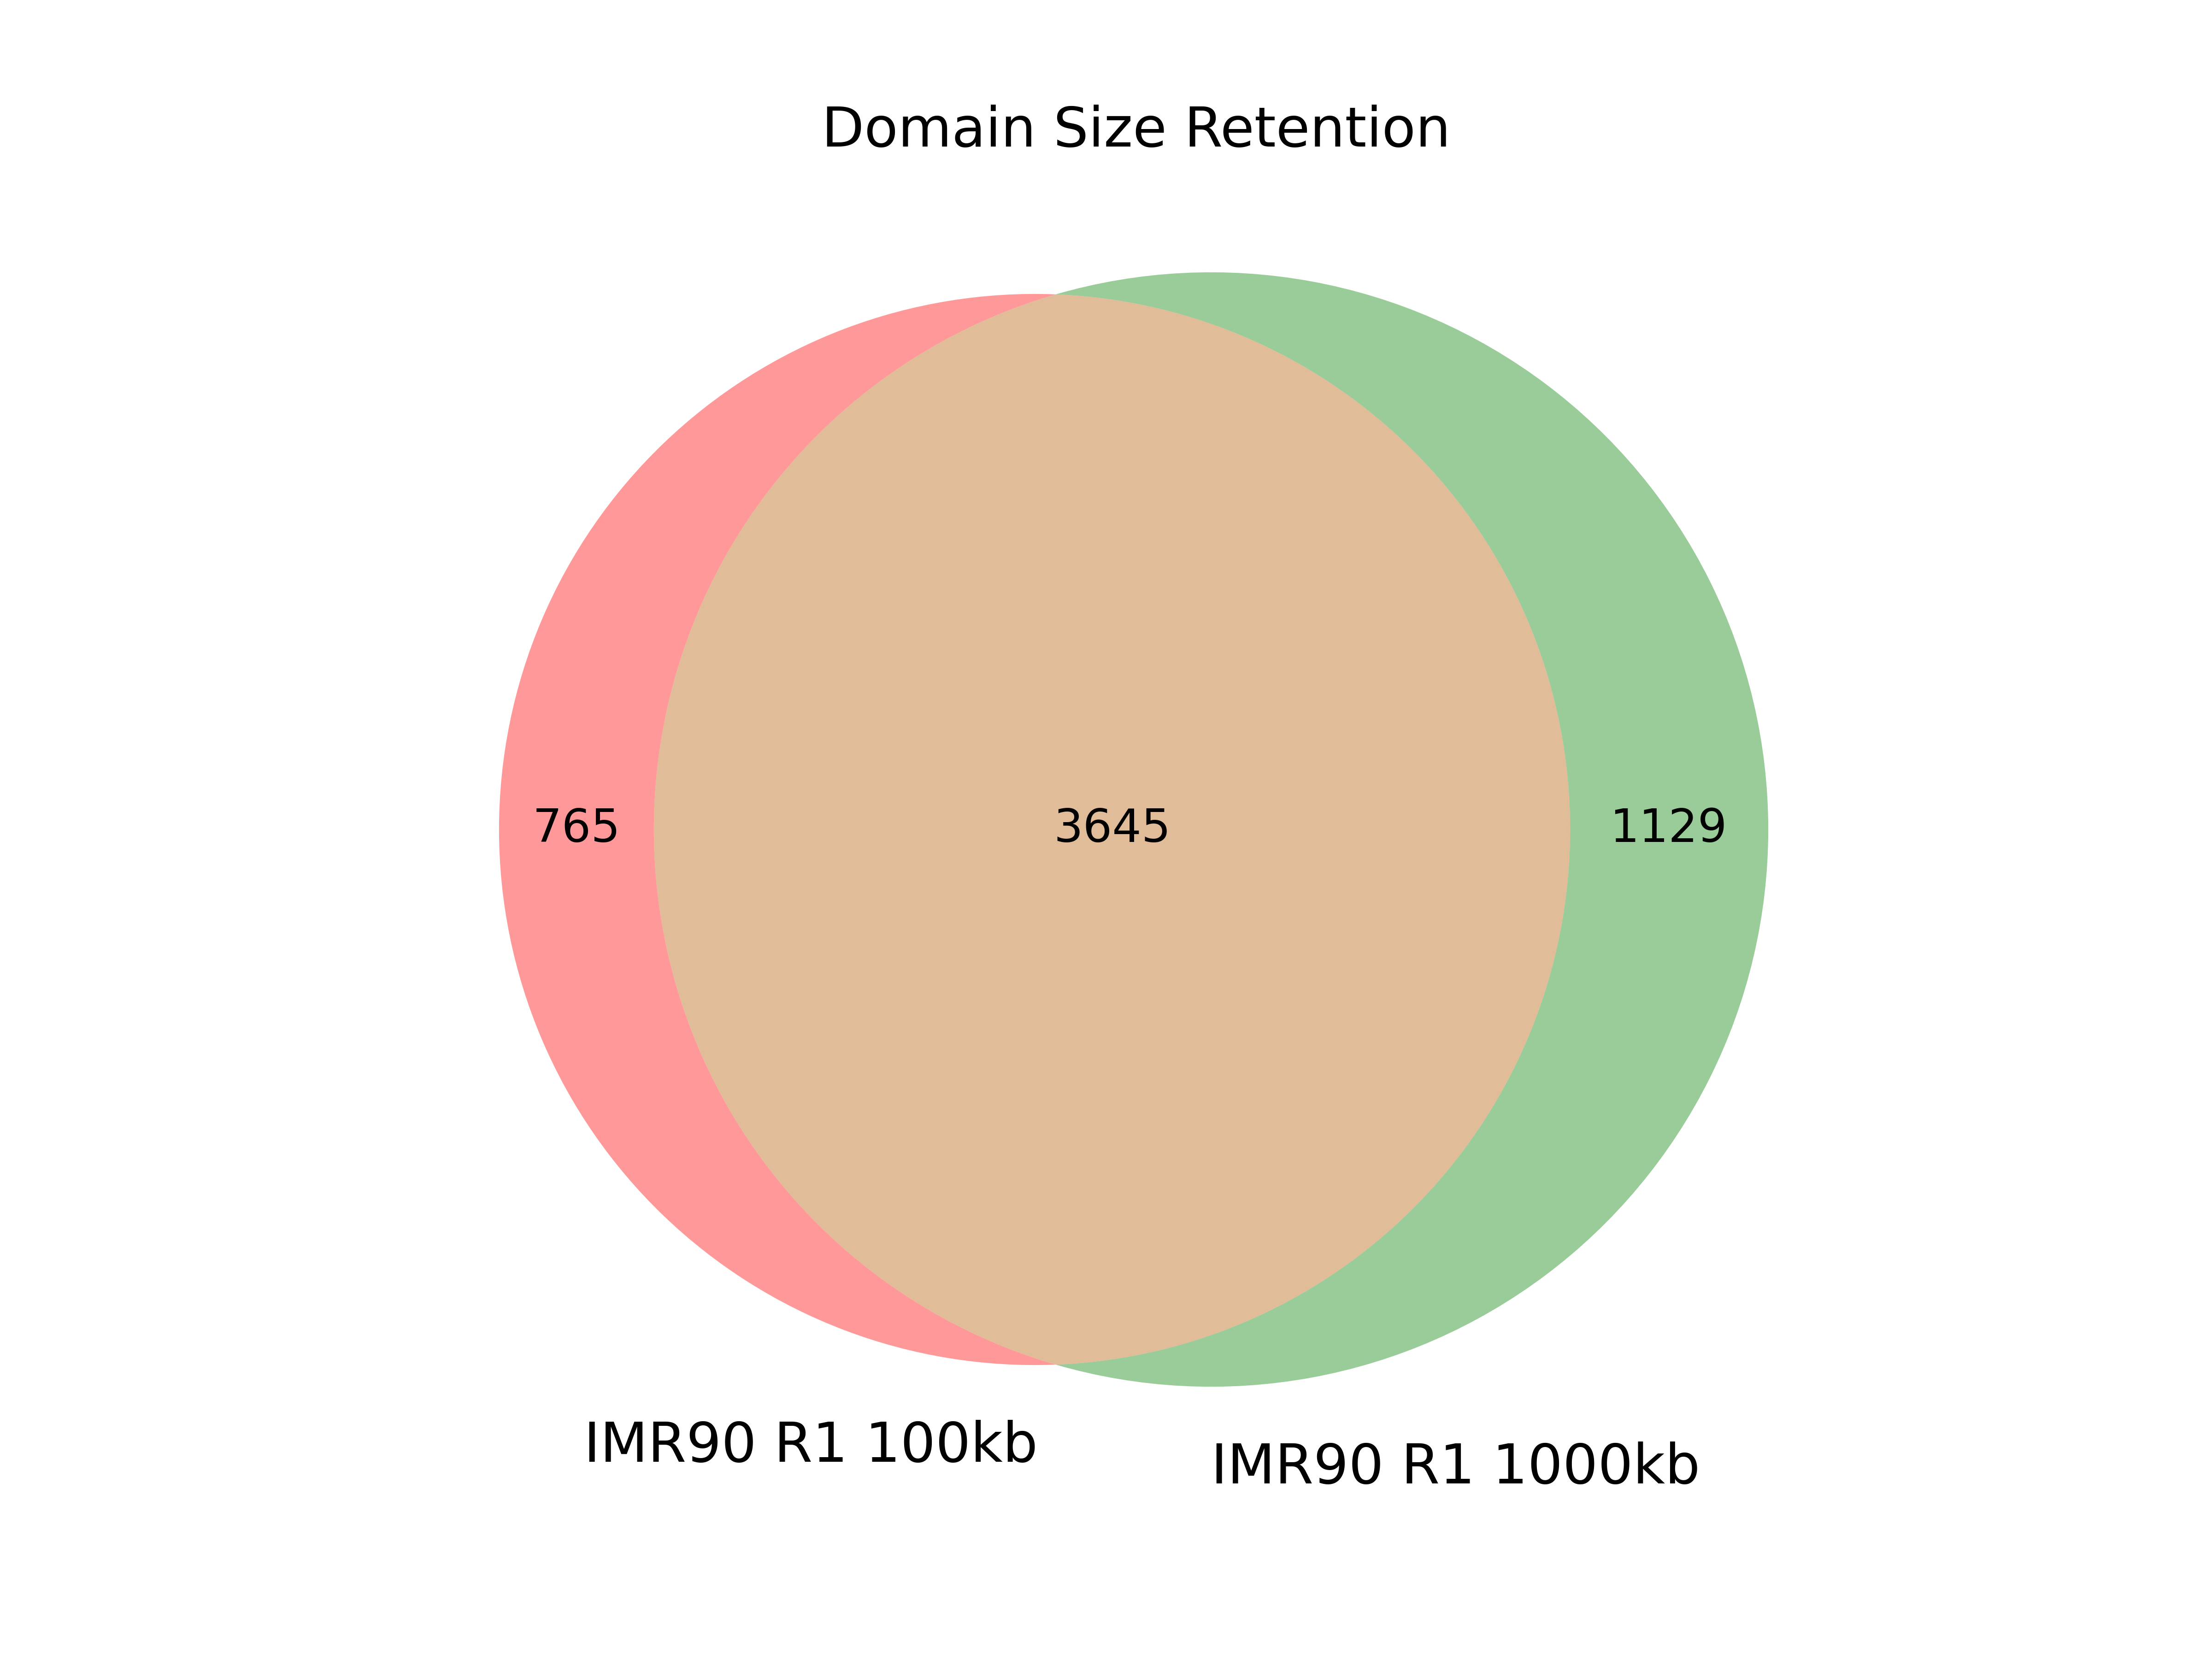
\includegraphics[width=\textwidth]{./figures/supplementary/domains/venn2_ir1_100kb_vs_ir1_1000kb.png}
  \end{minipage}
\end{figure}

\newpage

\subsection*{Domain Overlaps with Lesions}

\begin{figure}[thp]
  \centering
  \caption{Domain Overlaps by Window Size}
  \begin{minipage}{0.45\textwidth}%
    \centering
    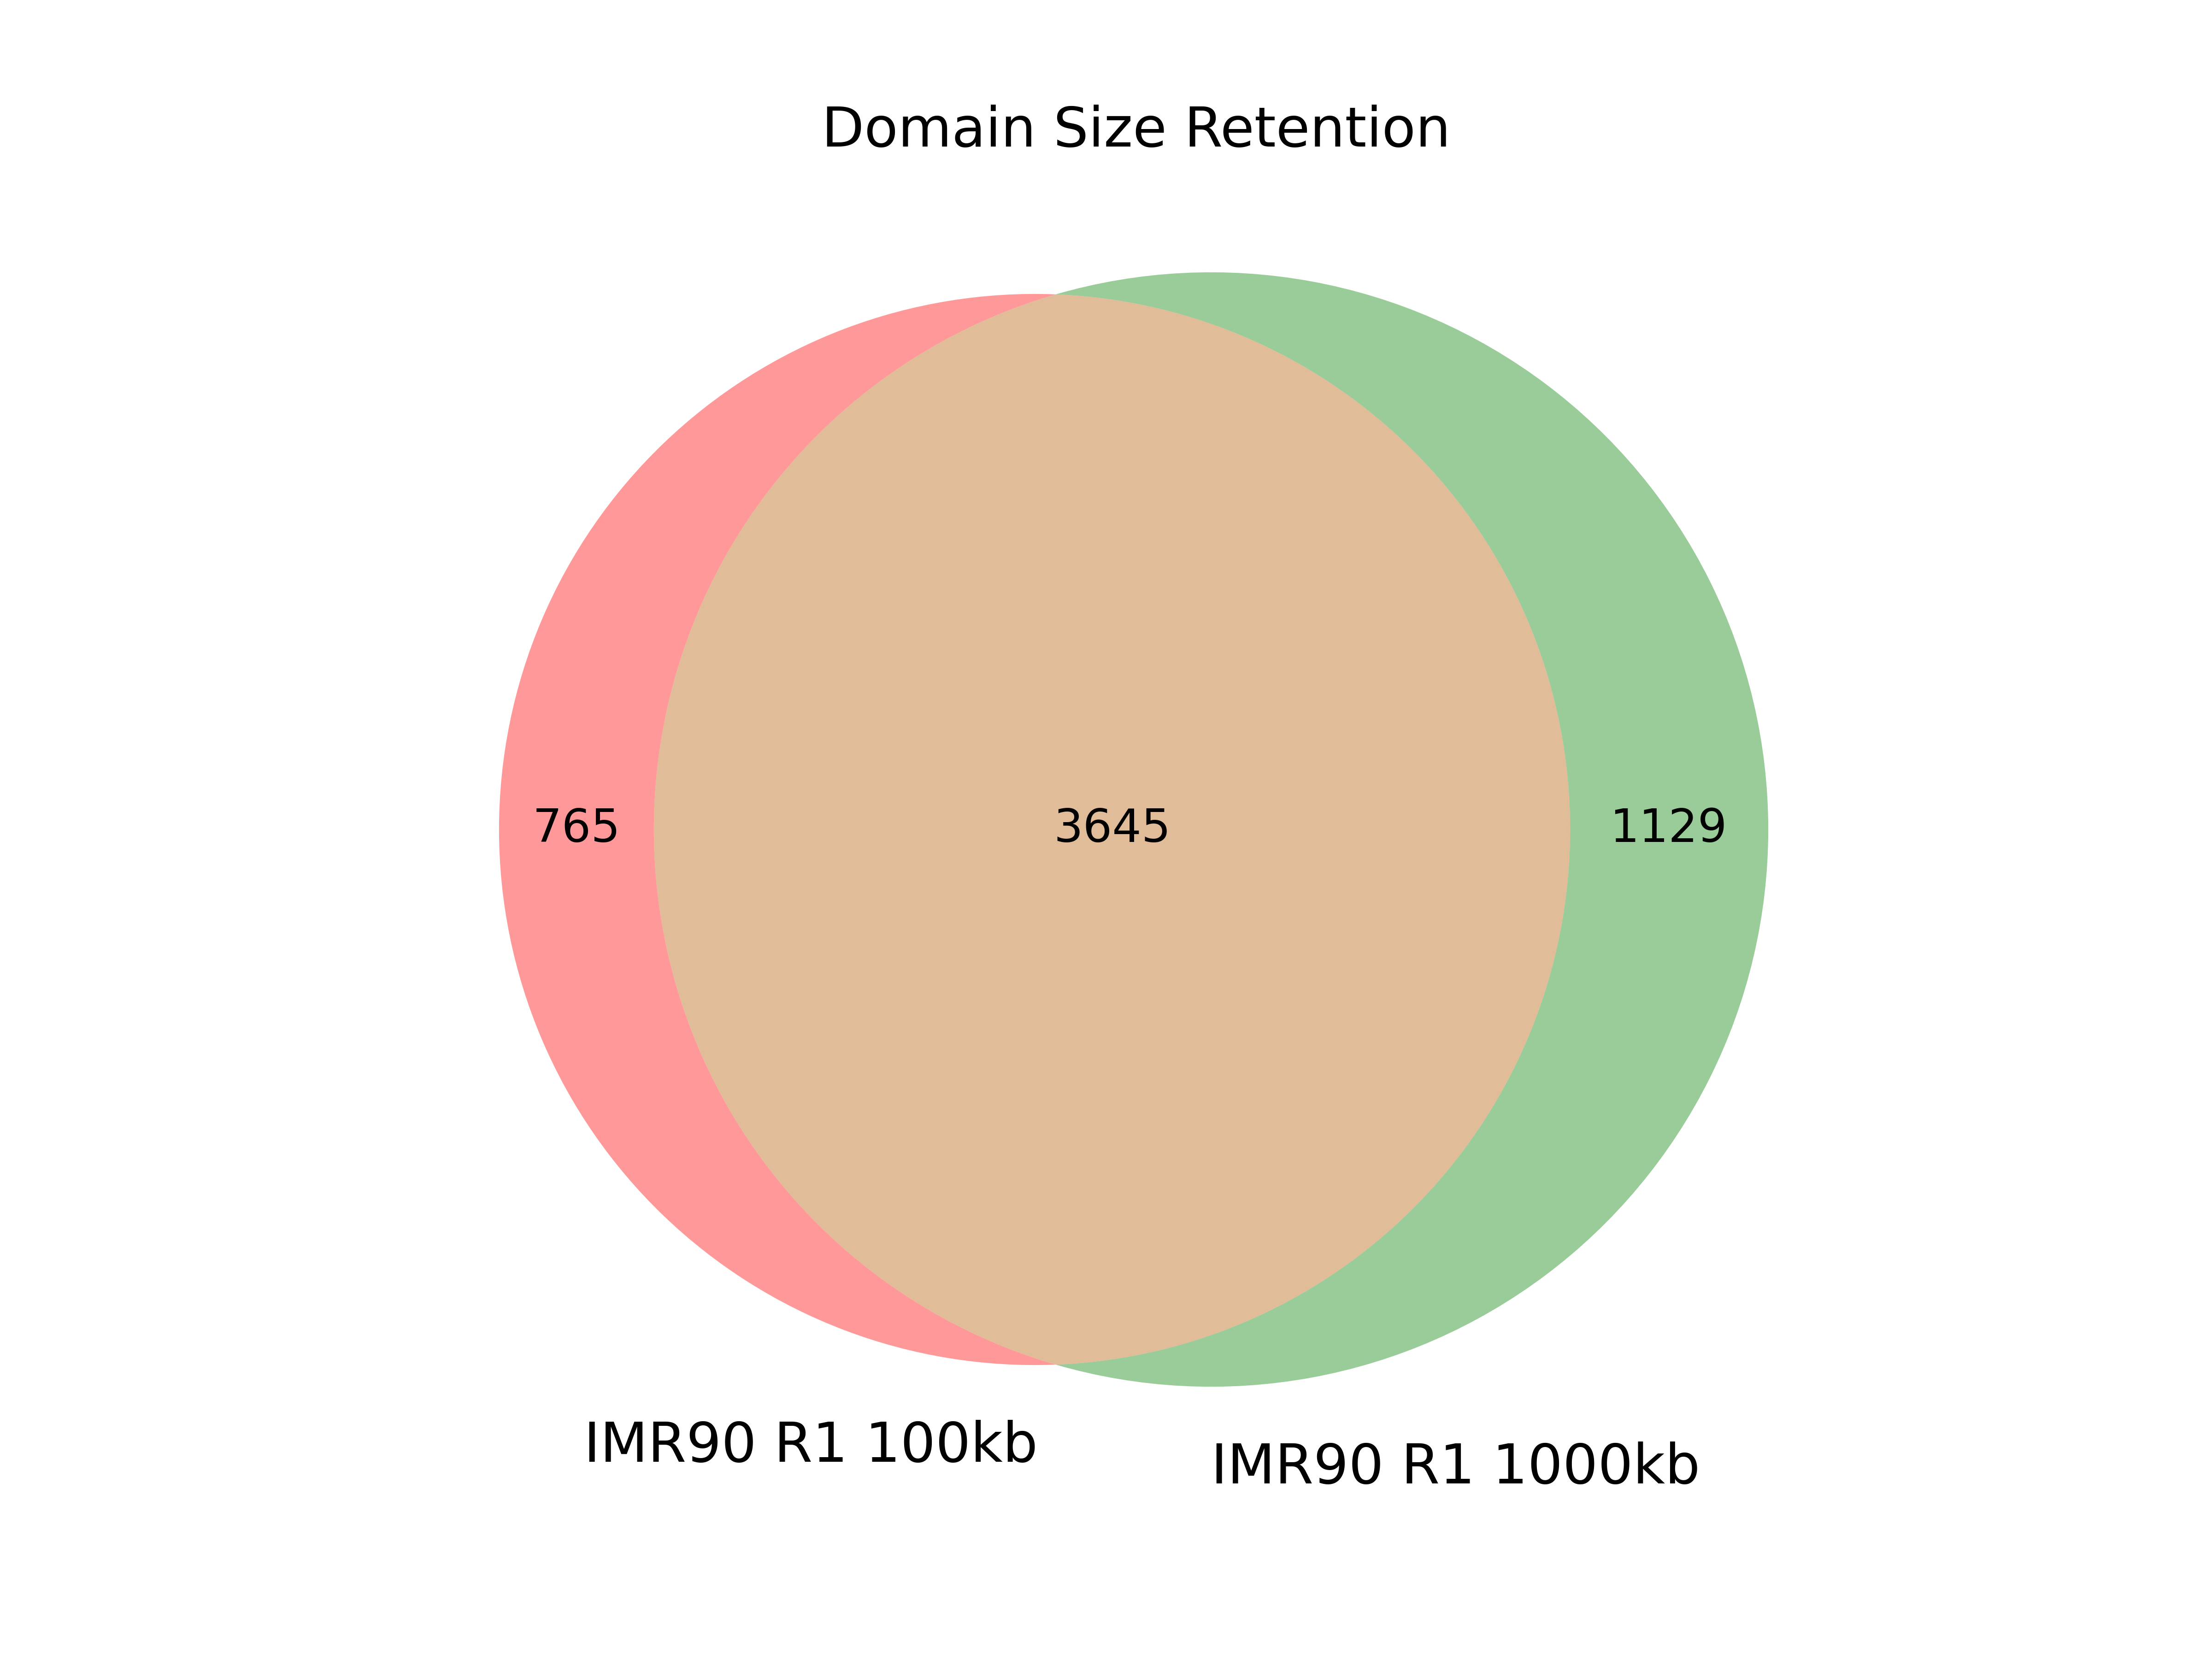
\includegraphics[width=\textwidth]{./figures/supplementary/domains/venn2_ir1_100kb_vs_ir1_1000kb.png}
  \end{minipage}

  \hfill

  \begin{minipage}{0.45\textwidth}
    \centering
    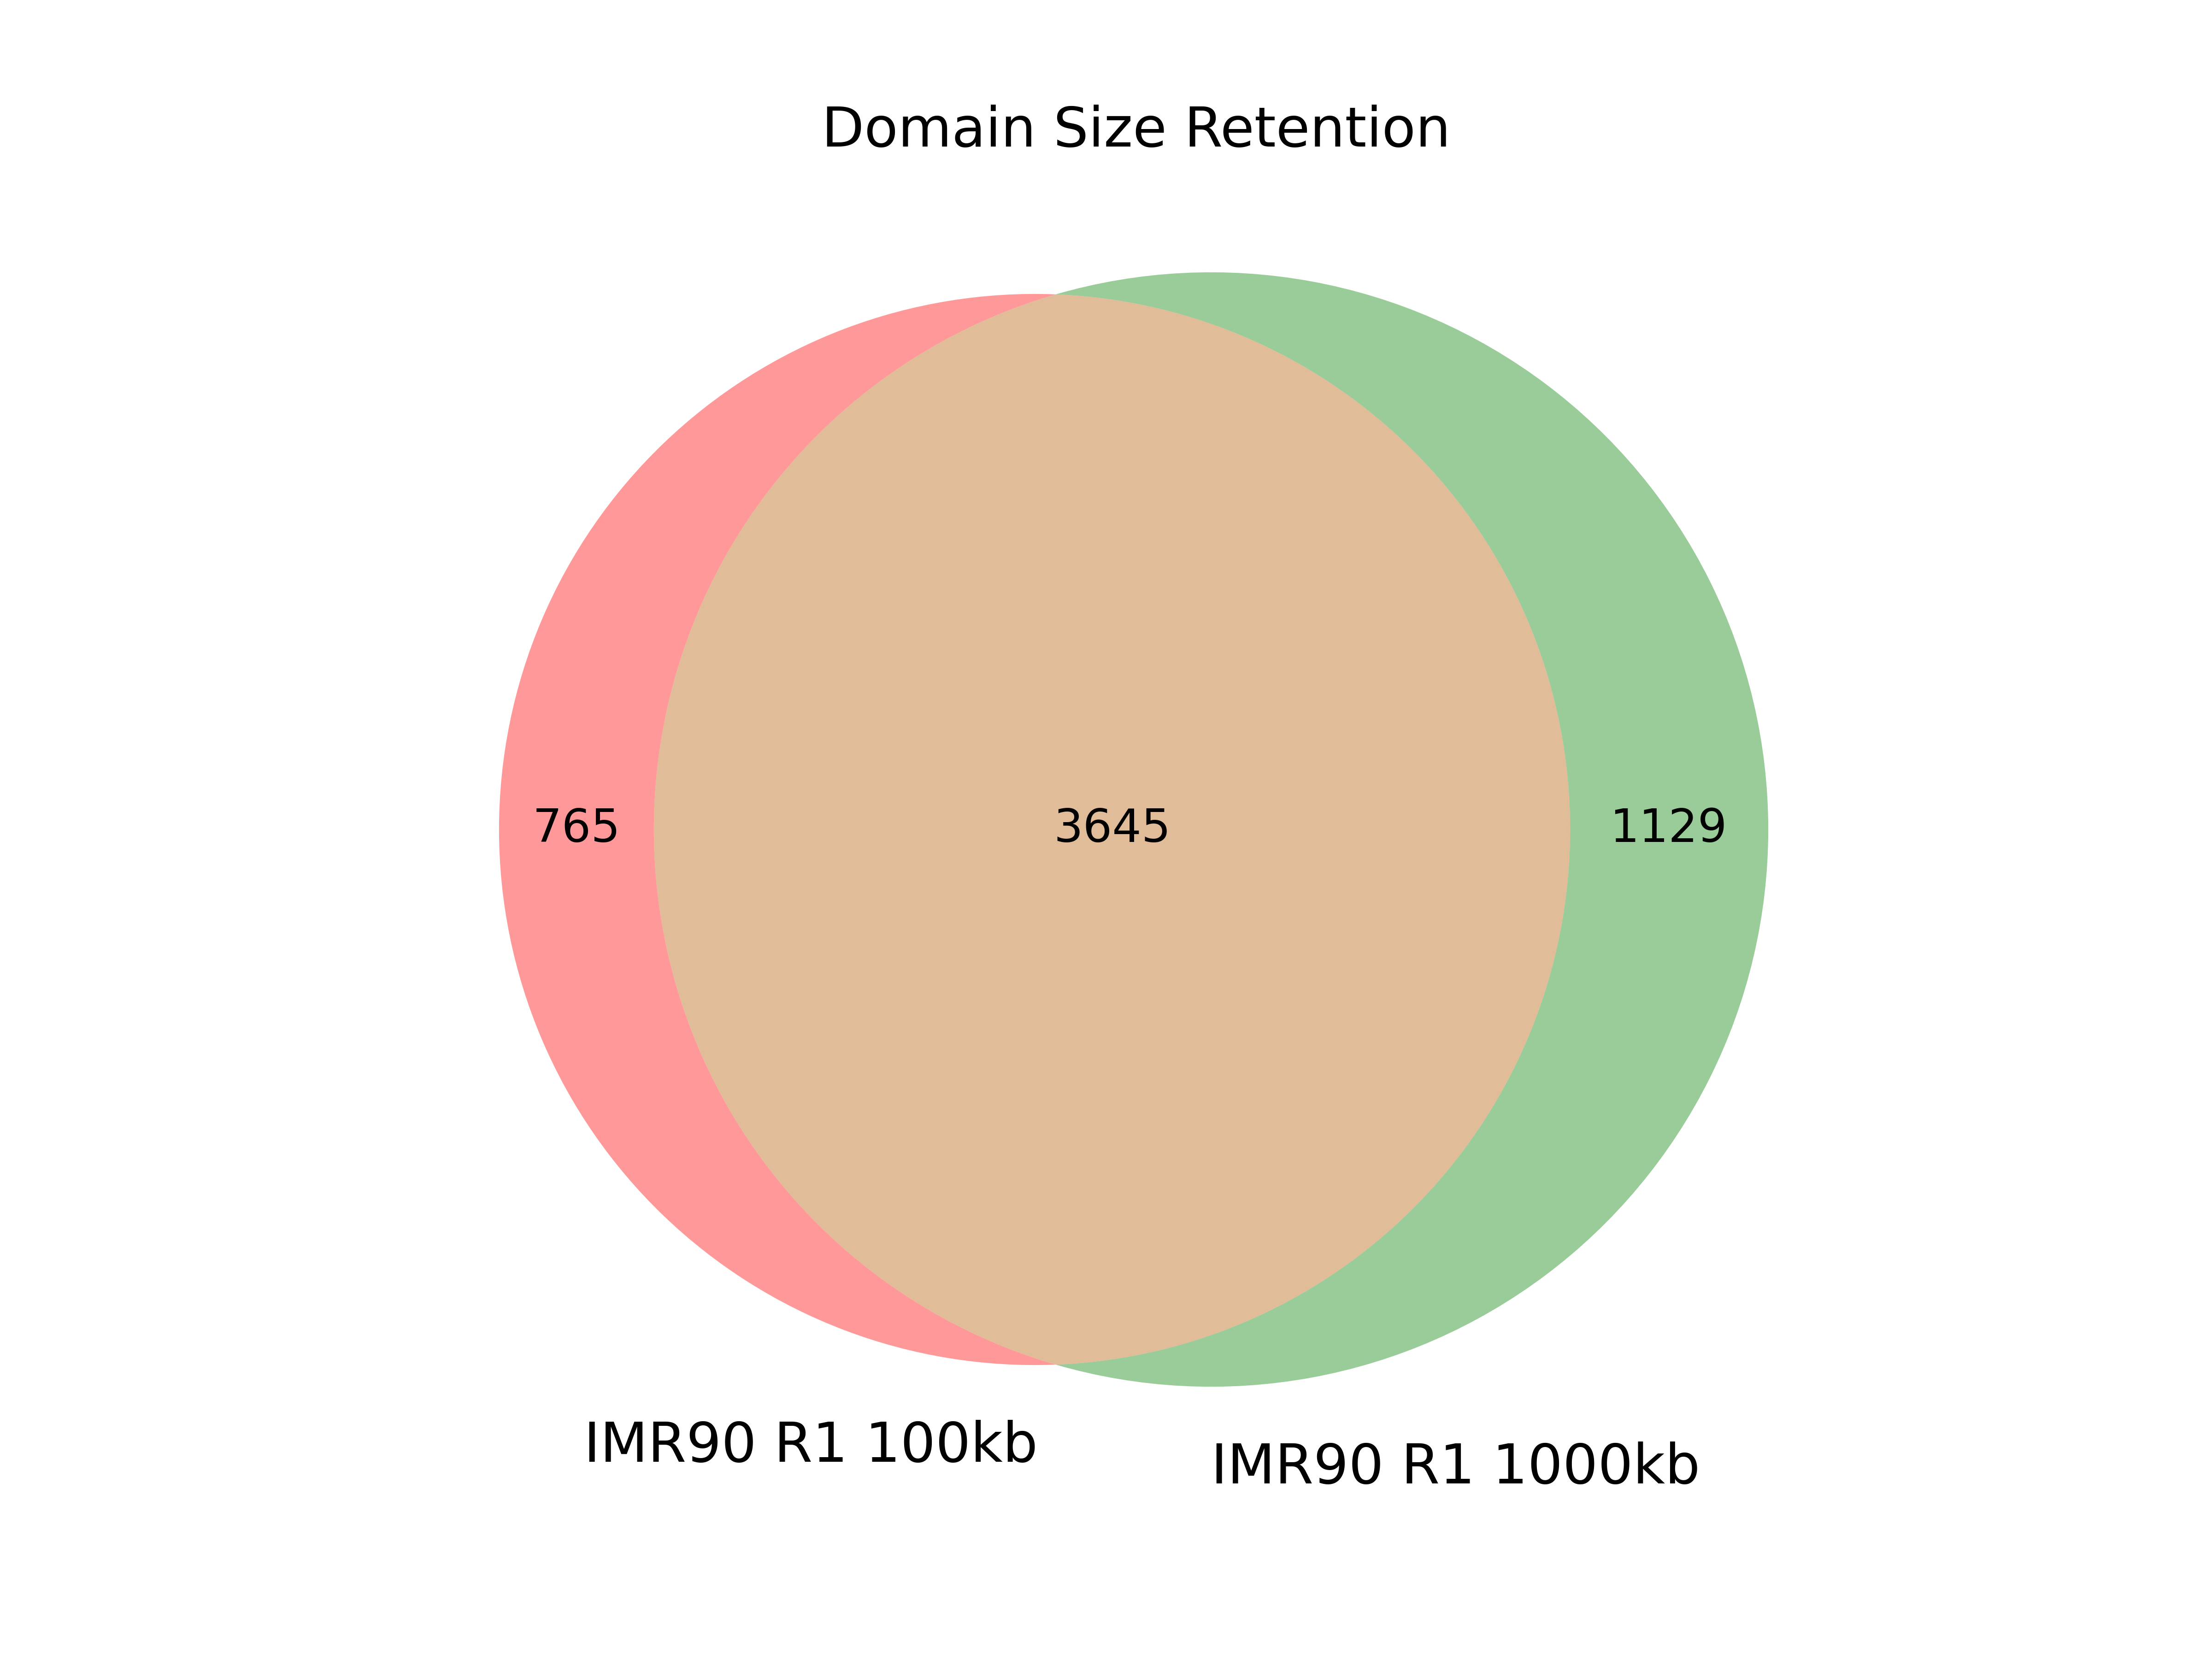
\includegraphics[width=\textwidth]{./figures/supplementary/domains/venn2_ir1_100kb_vs_ir1_1000kb.png}
  \end{minipage}
\end{figure}
